
El detector CMS, representado de manera esquem\'atica en la Figura~\ref{fig:CMS}, se localiza en uno de los puntos del acelerador LHC donde se hacen colisionar los haces de protones. Est\'a compuesto, de la zona m\'as interna a la m\'as externa, por un tracker de p\'ixeles y tiras (strips) de silicio para la detecci\'n de partículas cargadas con gran resoluci\'on espacial, un calor\'metro electromagn\'etico de cristal de tungstato (ECAL) para la medida de electrones y fotones principalmente, un calor\'imetro hadr\'onico constituido de material denso y absorbente (HCAL) especializado en la medida de hadrones, y finalmente, en la parte m\'as externa se encuentran las c\'amaras de muones. Entre el HCAL y las c\'amaras de muones se tiene un im\'an superconductor que alcanza un campo magn\'etico de 3.8 T, suficiente para curvar part\'iculas cargadas de muy alto momento y permitir una buena resoluci\'on en la medida del mismo.

En cuanto a su geometr\'ia, el sistema de coordenadas aceptado tiene como origen el punto de colisi\'on, el eje y apunta verticalmente hacia arriba, el eje x radialmente desde el origen, y el eje z recorre la direcci\'on del haz (ver Figura~\ref{fig:CMS}). El \'angulo azimutal $\phi$ se mide a partir del eje x en el plano x-y transverso al haz, mientras que el \'angulo polar $\theta$ desde el eje z en el plano x-z. Otra variable angular importante que ser\'a utilizada en el an\'alisis por ser invariante bajo transformaciones de Lorentz en el eje z, es la pseudorrapidez $\eta$, que se define en funci\'on del \'angulo polar como:

\begin{equation}
  \eta = -\ln\left(\tan\dfrac{\theta}{2}\right)
\label{eq:eta}
\end{equation}

\begin{figure}
\centering
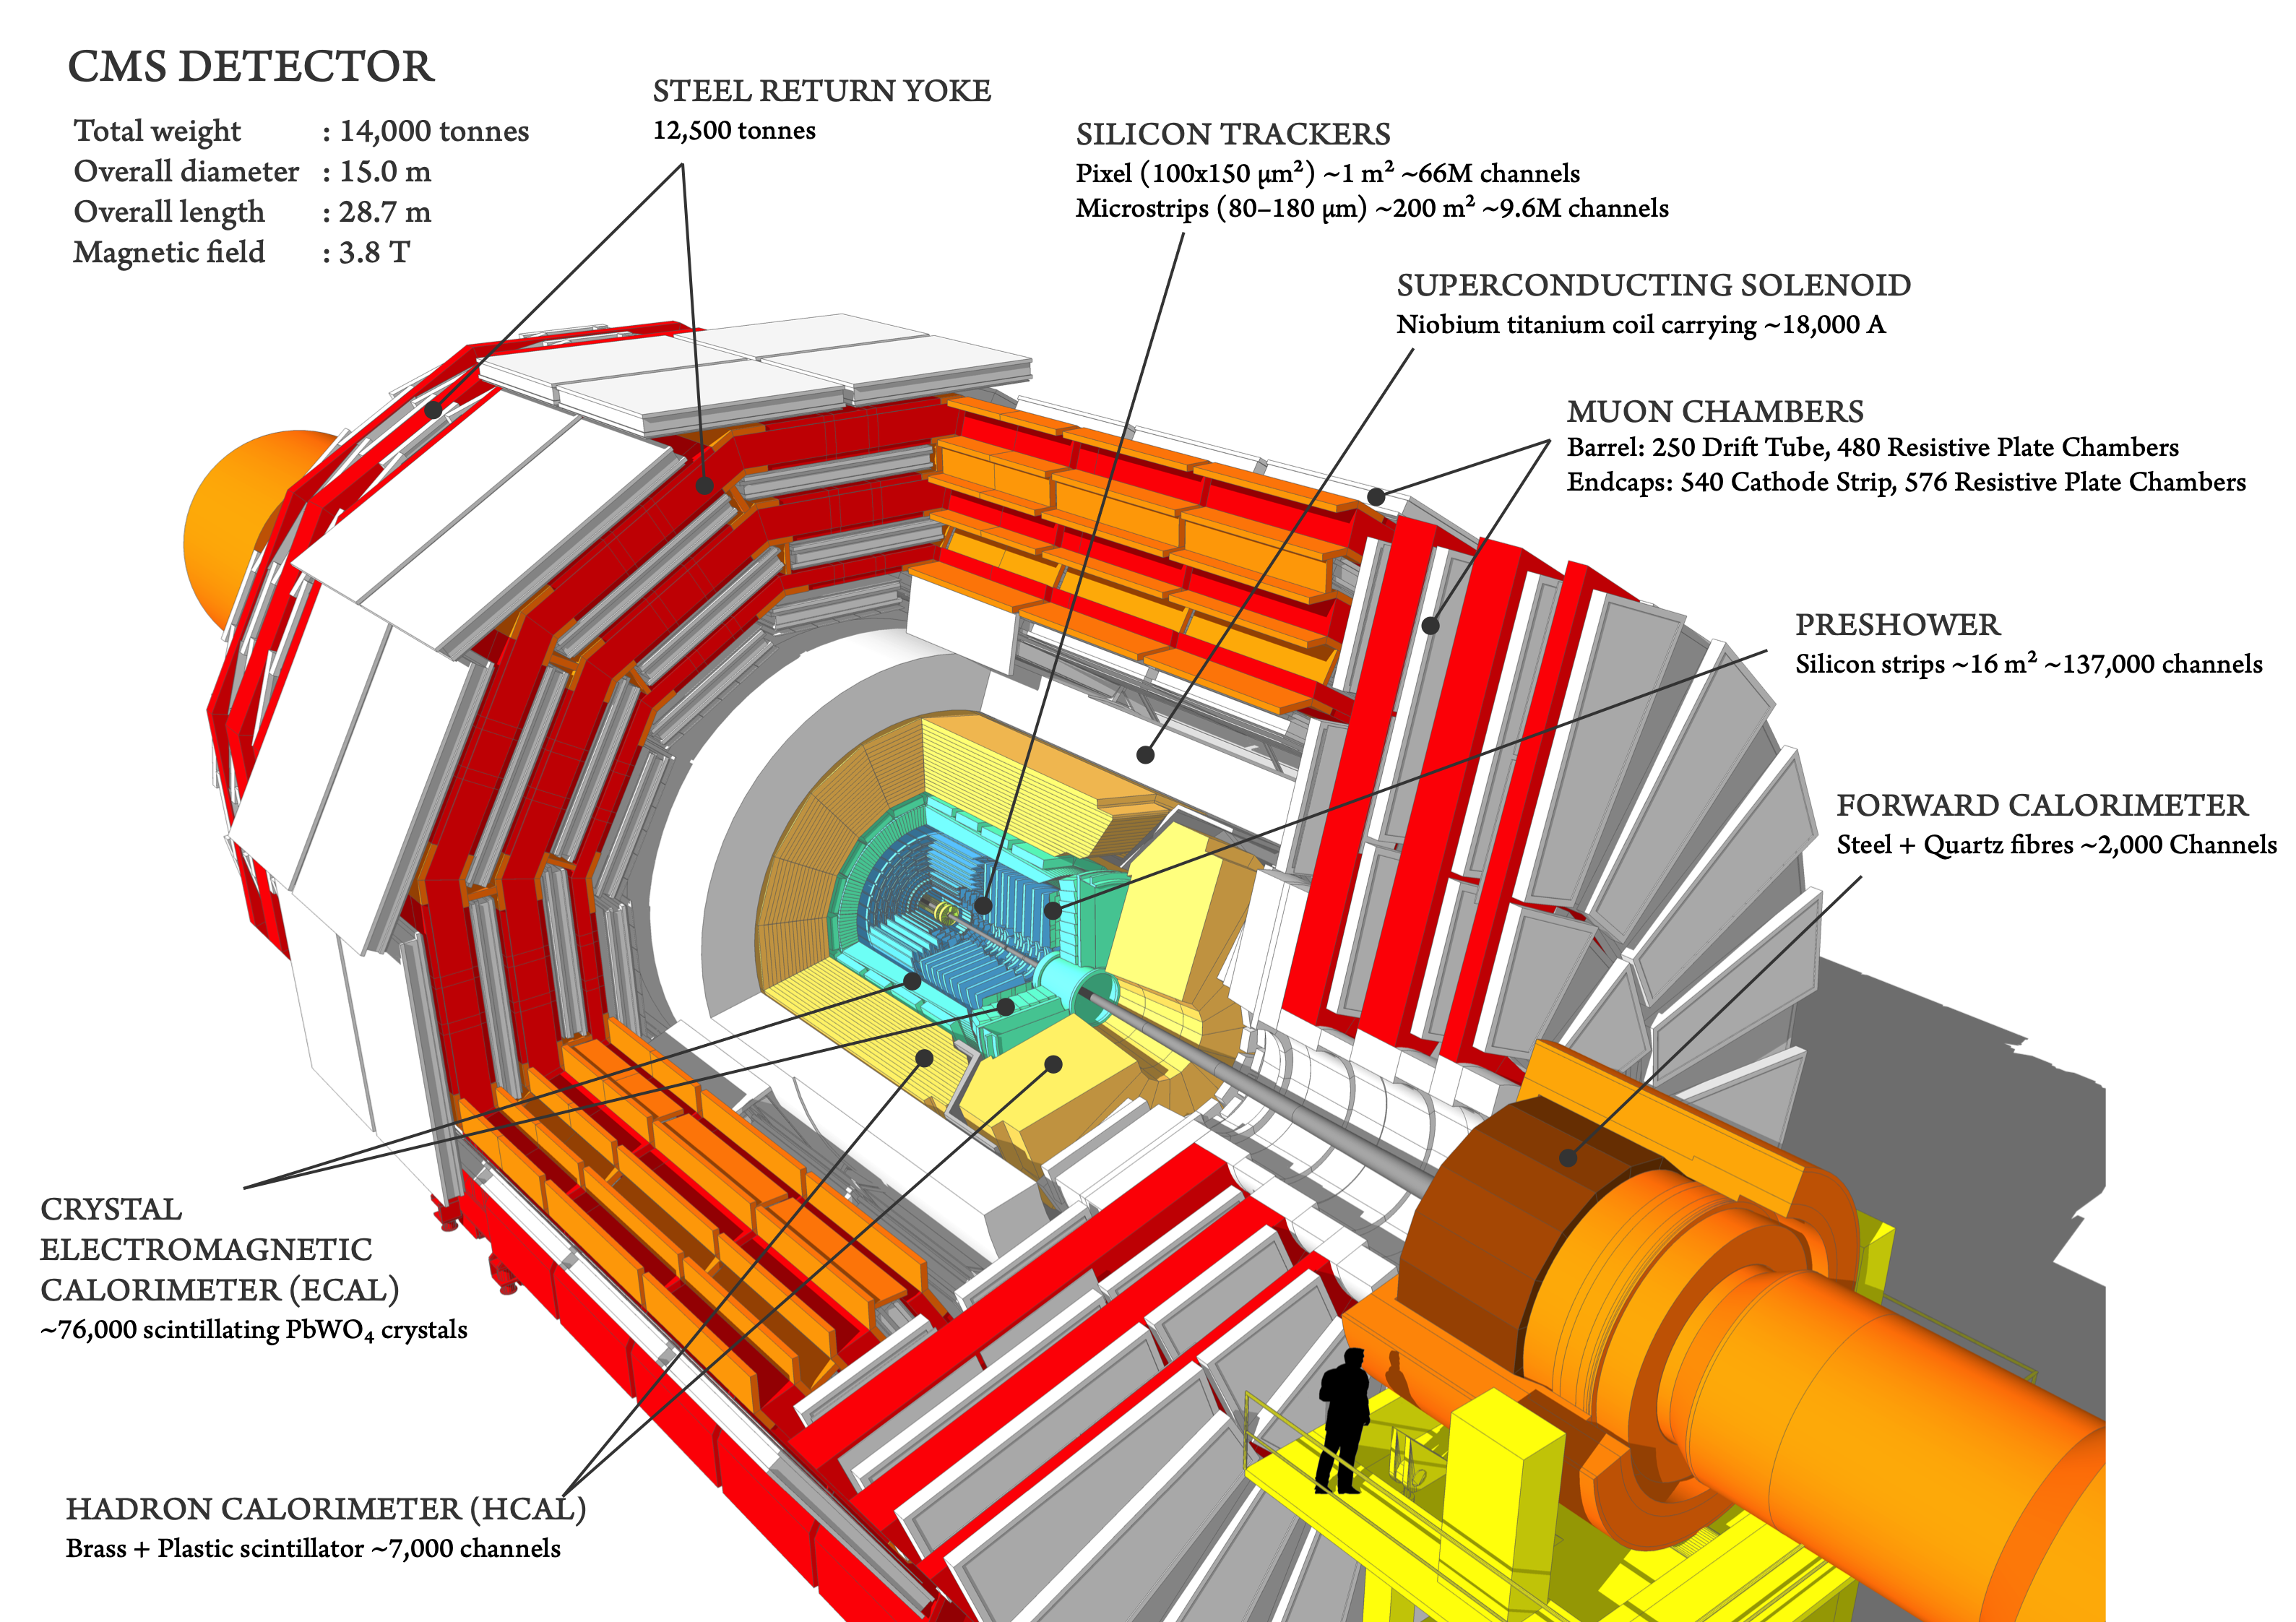
\includegraphics[width=0.80\textwidth]{figures/cms_160312_02.png}
\caption{Representaci\'on gr\'afica de las distintas partes del detector CMS. Imagen tomada de \cite{CMSplot}.}
\label{fig:CMS}        
\end{figure}


De esta manera, se suelen usar variables definidas en el plano transversal a la dirección del haz de partículas como el momento transverso $p_{T}$ o la energía transversa $E_{T}$. 

En este trabajo nos centraremos en la medida de los muones, que al ser part\'iculas cargadas dejan señal en el tracker interno, no interaccionan apenas con el material denso de los calor\'imetros, y llegan a las c\'amaras de muones externas, situadas a unos cuatro metros del punto de colisi\'on. En las siguientes subsecciones se describir\'an dos de los subdetectores que componen las c\'amaras de muones que ser\'an utilizados en el an\'alisis: los Drift Tubes (DTs), y los Cathode Strip Chambers (CSCs).

\subsection{Drift Tubes: DTs}\label{sec:DTs}


\begin{figure}
\centering
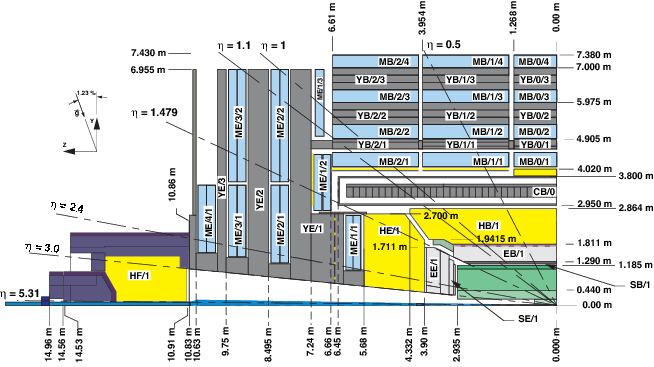
\includegraphics[width=0.8\textwidth]{figures/CMSview1.png}
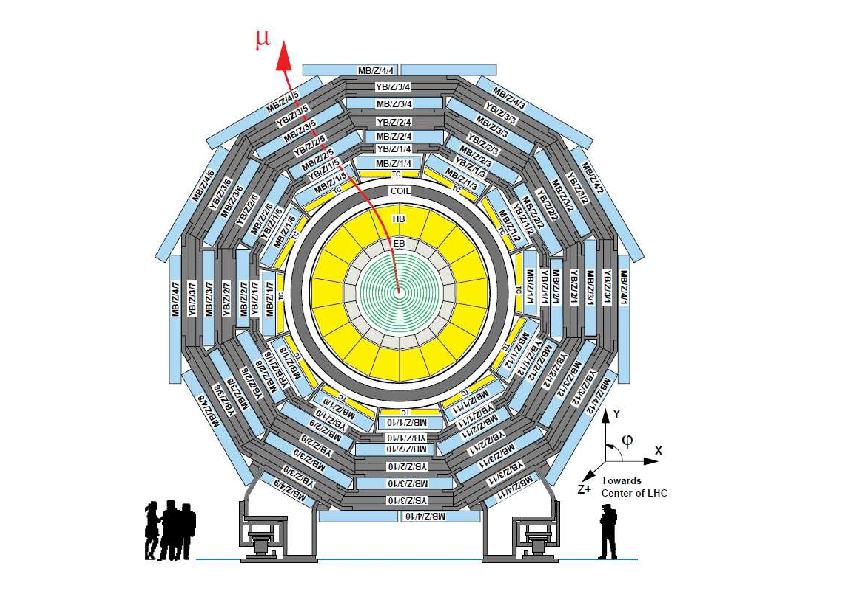
\includegraphics[width=0.8\textwidth]{figures/CMSview.png}
\caption{Vista esquem\'atica del detector CMS. Izquierda: vista longitudinal de un cuarto del detector. Derecha: vista transversal en $z = 0$. Ambas figuras han sido tomadas de \cite{DTperformance}}
\label{fig:CMSsub}
\end{figure}



\cite{DTperformance}

\subsection{Cathode Strip Chambers: CSCs}\label{sec:CSCs}

\cite{CSCperformance}
